% Template for Elsevier CRC journal article
% version 1.2 dated 09 May 2011

% This file (c) 2009-2011 Elsevier Ltd.  Modifications may be freely made,
% provided the edited file is saved under a different name

% This file contains modifications for Procedia CIRP

% Changes since version 1.1
% - added "procedia" option compliant with ecrc.sty version 1.2a
%   (makes the layout approximately the same as the Word CRC template)
% - added example for generating copyright line in abstract

%-----------------------------------------------------------------------------------

%% This template uses the elsarticle.cls document class and the extension package ecrc.sty
%% For full documentation on usage of elsarticle.cls, consult the documentation "elsdoc.pdf"
%% Further resources available at http://www.elsevier.com/latex

%-----------------------------------------------------------------------------------

%%%%%%%%%%%%%%%%%%%%%%%%%%%%%%%%%%%%%%%%%%%%%%%%%%%%%%%%%%%%%%
%%%%%%%%%%%%%%%%%%%%%%%%%%%%%%%%%%%%%%%%%%%%%%%%%%%%%%%%%%%%%%
%%                                                          %%
%% Important note on usage                                  %%
%% -----------------------                                  %%
%% This file should normally be compiled with PDFLaTeX      %%
%% Using standard LaTeX should work but may produce clashes %%
%%                                                          %%
%%%%%%%%%%%%%%%%%%%%%%%%%%%%%%%%%%%%%%%%%%%%%%%%%%%%%%%%%%%%%%
%%%%%%%%%%%%%%%%%%%%%%%%%%%%%%%%%%%%%%%%%%%%%%%%%%%%%%%%%%%%%%

%% The '3p' and 'times' class options of elsarticle are used for Elsevier CRC
%% The 'procedia' option causes ecrc to approximate to the Word template
\documentclass[3p,times,procedia,twocolumn,twoside]{elsarticle}
\flushbottom

%% The `ecrc' package must be called to make the CRC functionality available
\usepackage{ecrc,stfloats}
%\usepackage{amsmath}


%% The ecrc package defines commands needed for running heads and logos.
%% For running heads, you can set the journal name, the volume, the starting page and the authors

%% set the volume if you know. Otherwise `00'
\volume{00}

%% set the starting page if not 1
\firstpage{1}

%% Give the name of the journal
\journalname{Procedia CIRP}

%% Give the author list to appear in the running head
%% Example \runauth{C.V. Radhakrishnan et al.}
\runauth{Author name}

%% The choice of journal logo is determined by the \jid and \jnltitlelogo commands.
%% A user-supplied logo with the name <\jid>logo.pdf will be inserted if present.
%% e.g. if \jid{yspmi} the system will look for a file yspmilogo.pdf
%% Otherwise the content of \jnltitlelogo will be set between horizontal lines as a default logo

%% Give the abbreviation of the Journal.
\jid{cirp}

%% Give a short journal name for the dummy logo (if needed)
%\jnltitlelogo{Procedia CIRP}

%% Hereafter the template follows `elsarticle'.
%% For more details see the existing template files elsarticle-template-harv.tex and elsarticle-template-num.tex.

%% Elsevier CRC generally uses a numbered reference style
%% For this, the conventions of elsarticle-template-num.tex should be followed (included below)
%% If using BibTeX, use the style file elsarticle-num.bst

%% End of ecrc-specific commands
%%%%%%%%%%%%%%%%%%%%%%%%%%%%%%%%%%%%%%%%%%%%%%%%%%%%%%%%%%%%%%%%%%%%%%%%%%

%% The amssymb package provides various useful mathematical symbols

\usepackage{amssymb}
\usepackage{gensymb}
\usepackage{amsmath}

%% The amsthm package provides extended theorem environments
%% \usepackage{amsthm}

%% The lineno packages adds line numbers. Start line numbering with
%% \begin{linenumbers}, end it with \end{linenumbers}. Or switch it on
%% for the whole article with \linenumbers after \end{frontmatter}.
%% \usepackage{lineno}

%% natbib.sty is loaded by default. However, natbib options can be
%% provided with \biboptions{...} command. Following options are
%% valid:

%%   round  -  round parentheses are used (default)
%%   square -  square brackets are used   [option]
%%   curly  -  curly braces are used      {option}
%%   angle  -  angle brackets are used    <option>
%%   semicolon  -  multiple citations separated by semi-colon
%%   colon  - same as semicolon, an earlier confusion
%%   comma  -  separated by comma
%%   numbers-  selects numerical citations
%%   super  -  numerical citations as superscripts
%%   sort   -  sorts multiple citations according to order in ref. list
%%   sort&compress   -  like sort, but also compresses numerical citations
%%   compress - compresses without sorting
%%
\biboptions{sort&compress}

% \biboptions{}

% if you have landscape tables
\usepackage[figuresright]{rotating}
%\usepackage{harvard}
% put your own definitions here:x
%   \newcommand{\cZ}{\cal{Z}}
%   \newtheorem{def}{Definition}[section]
%   ...

% add words to TeX's hyphenation exception list
%\hyphenation{author another created financial paper re-commend-ed Post-Script}

% declarations for front matter
\usepackage{fleqn}
\mathindent0pt
\parskip0pt
\begin{document}

\begin{frontmatter}

%% Title, authors and addresses

%% use the tnoteref command within \title for footnotes;
%% use the tnotetext command for the associated footnote;
%% use the fnref command within \author or \address for footnotes;
%% use the fntext command for the associated footnote;
%% use the corref command within \author for corresponding author footnotes;
%% use the cortext command for the associated footnote;
%% use the ead command for the email address,
%% and the form \ead[url] for the home page:
%%
%% \title{Title\tnoteref{label1}}
%% \tnotetext[label1]{}
%% \author{Name\corref{cor1}\fnref{label2}}
%% \ead{email address}
%% \ead[url]{home page}
%% \fntext[label2]{}
%% \cortext[cor1]{}
%% \address{Address\fnref{label3}}
%% \fntext[label3]{}

\dochead{10th CIRP Conference on Industrial Product-Service Systems, IPS$^{2}$ 2018, 29-31 May 2018,\\ Link\"oping, Sweden}
%% Use \dochead if there is an article header, e.g. \dochead{Short communication}
%% \dochead can also be used to include a conference title, if directed by the editors
%% e.g. \dochead{17th International Conference on Dynamical Processes in Excited States of Solids}

\title{Data based optimization of the operation of industrial chillers}

%% use optional labels to link authors explicitly to addresses:
%% \author[label1,label2]{<author name>}
%% \address[label1]{<address>}
%% \address[label2]{<address>}



\author[a,*]{Benjamin M\"orzinger}
\author[a]{Christoph Loschan}
\author[a]{Florian Kloibhofer}
\author[a]{Friedrich Bleicher}

\address[a]{Institute for Production Engineering and Laser Technology, TU Wien, Getreidemarkt 9, Vienna, 1060, Austria}

\begin{abstract}
%% Text of abstract
Click here and insert your abstract text.
\end{abstract}

\begin{keyword}
Type your keywords here, separated by semicolons ;

%% keywords here, in the form: keyword \sep keyword

%% PACS codes here, in the form: \PACS code \sep code

%% MSC codes here, in the form: \MSC code \sep code
%% or \MSC[2008] code \sep code (2000 is the default)
\end{keyword}
\CorText[cor1]{Benjamin M\"orzinger. Tel.: +0043-1-58801-31118; fax: +0043-1-58801-931118.\email{moerzinger@ift.at}}
\belowfrontmatterskip0pt
\end{frontmatter}

%\correspondingauthor[*]{Corresponding author. Tel.: +0-000-000-0000 ; fax: +0-000-000-0000.}


%%
%% Start line numbering here if you want
%%
% \linenumbers

%% main text


\section{Introduction}
\label{main}
The manufacturing industry is one of societies’ largest energy consumers. In the European Union it accounts for 26\% of the total final energy consumption \cite{Eurostata}. Hence, successful energy efficiency measures in this sector would lead to a major reduction in the overall demand. The achievable savings in this sector amount to between 30\% and 65\%, according to \cite{Bonneville2006a}. Furthermore, in \cite{Paulus2011} opportunities for balancing the electrical energy market via demand side management of large- scale industrial enterprises where identified. In the past, the factors cost, time, quality and flexibility identified by \cite{Chryssolouris1992} have been the most common basis for decisions in manufacturing.  Rising legislative pressure as well as foreseeable resource shortages and increasing awareness in the general public force the industry to reduce energy demand and CO\textsubscript{2} emissions. Several approaches for systematic energy efficiency improvements have been developed \cite{Thiede2012,Introna2014,May2015,Kovacic2013}. Existing approaches however tend to tackle only limited parts of the production process \cite{Herrmann2011,Kara2011,Weinert2011} and therefore fall short at achieving the necessary savings. In order to maximise those, all relevant areas of a given production facility need to be taken into consideration. In the case of production engineering, this does not only involve production machines, but also energy systems, the building and elements concerned with the material flow (logistics) \cite{Hesselbach2008,Bleicher2014a}. In order to choose and evaluate energy efficiency measures and select the most promising ones, not only their effect on energy demand, but also on the production process itself need to be predicted.\\
Following the concept of Cyber-Physical systems (CPS) in the context of manufacturing systems and Industry 4.0 as discussed in \cite{Jazdi2014,Monostori2014} we propose a complementary method regarding the incorporation of energy use into industrial planning processes: the Balanced Manufacturing Method. In this paper, we illustrate the application of this method in the context of the optimization of the operation of industrial chillers. Based on monitoring data, models are derived and combined to a virtual representation of the real system. The resulting simulation is then used to optimize the operation strategy. The result of this process is then returned to be applied to the physical systems.\\
This paper is structured as follows: in the following chapter the general method is explained. Then, the model parametrization, simulation implementation and finally the optimization is described. A full documentation of the findings, including a description of the methodology and an interactive demonstrator of the developed tool can be found at: http://bama.ift.tuwien.ac.at.
\section{BaMa Method}
Balanced Manufacturing (BaMa) tries to deliver plant operation strategies, planning and control that not only consider the conventional success factors, but also include energy demand and energy related CO\textsubscript{2}-emissions as evaluation-criteria. Compared to other energy management tools, there are two main differences: The first is its holistic approach. Energy demand in production facilities is determined by several different parts of the plant. The relevant subsystems in this respect can be assigned to one of the categories: buildings, energy systems, production machines or logistics \cite{Leobner2015}. In order to exploit the full optimization potential, it is necessary to analyse not only the interaction of subsystems within a given category, but also the cross-category interaction. The second is that BaMa is not focused on the design of new facilities. It rather is a tool to optimize the operation of existing plants, although it can be used in the design phase as well. \\
BaMa consists of two main parts: First, the BaMa tool chain enabling the investigation and optimization of a given production plant. Second, a method for a thorough analysis of any given production facility. \linebreak This method is the basis for the tool chain and a standardized way to describe a production facility.\\
\subsection{Tool Chain}
\label{CHAP_ToolChain}
The BaMa Tool Chain contains three core modules. Based on information about the plant a simulation\linebreak model of the production site is established. This virtual representation of the real world stands at the core of the BaMa tool chain. In order to parametrize and validate the model, monitoring data from the production site can be used in the simulation and operation strategies generated through simulation can be sent to the control system of the shop floor. Deviations between expectation and reality can be used to enhance the model and increase the reliability and accuracy.  With the simulation model as a basis the BaMa tool chain consists of three core modules: 
\begin{figure}
	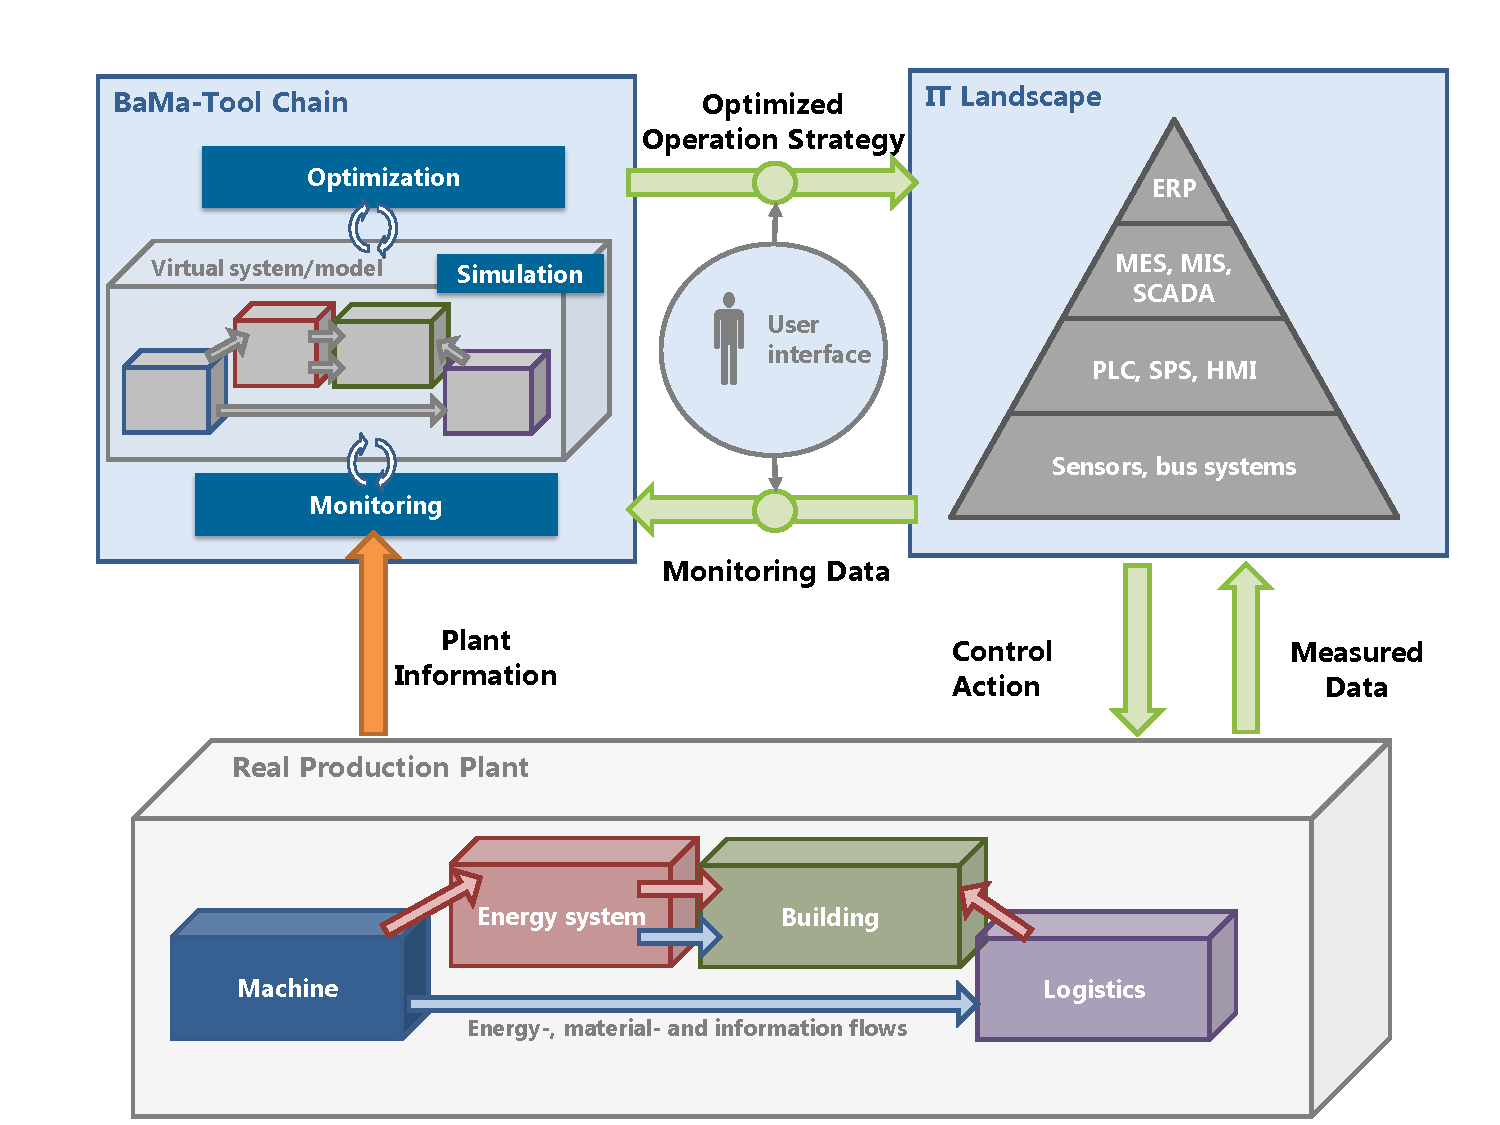
\includegraphics[width=0.5\textwidth]{figures/Architecture_new}
	\caption{BaMa Architecture}
	\label{FIG_Architecture}
\end{figure}
\begin{itemize}
	\item{Monitoring: Structural plant information,\linebreak sensor data from the field level as well as other information from the IT-landscape (e.g. from enterprise resource planning or manufacturing execution systems)  is aggregated and visualized. Results are used as report documents, which makes BaMa compatible with the requirements of the energy management standard ISO 50001. Furthermore, measured data is used as input for simulations as well as for the parametrization of the simulation models. According to \cite{monostori_cyber-physical_2014}, this intensive connection of embedded systems (sensors) with ongoing processes is among the main characteristics of CPS.}
	\item{Simulation/Prediction: Measured data and plant information are used to build a virtual representation of the production site. The resulting model allows forecasting of the overall energy demand based on a set of input parameters.}
	\item{Optimization: The evaluation of the results of repeated simulations enables an optimization framework to find beneficial operation plans for the virtual plant. Optimization targets can, for example, be energy demand, time or costs. Restrictions such as resource availability will also be considered.}
\end{itemize}
Figure \ref{FIG_Architecture} shows the relationships between the proposed tool chain, the production site and the IT landscape. The conventional IT landscape is the link between the BaMa tool chain and the production site. It transmits all relevant data to the BaMa Monitoring module. Using monitoring data and other qualitative and quantitative information about the plant under consideration, the tool chain proposes an optimized operation strategy. This strategy is reviewed by a human supervisor. Afterwards, the operation strategy can be handed over to the IT landscape. The proposed and reviewed operation strategy is processed and  control commands could be sent to the respective system. In order for BaMa to unfold its full optimization potential, this process needs to be carried out and executed on a regular basis. Therefore, a high integration into existing automation systems is necessary. \\
As mentioned, within the tool chain a "virtual twin" of the real production plant (i.e. a model) is used to predict the behavior of the physical system. The potential modeling effort is considerable and needs to be minimized in order to make BaMa a feasible and applicable tool for companies. To address this, the cube concept is introduced and will be explained in the following section.
\subsection{The Cube Concept}
\label{CHAP_CubeConcept}
Each production site needs to be modeled individually in order to be able to generate valid optimization strategies. For BaMa to be feasible despite this issue, a high degree of model re-usability must be achieved. \cite{Balci2012,Setavoraphan2008} suggest decomposition at model design level when dealing with simulations of comparable scope.\\
Object-oriented software engineering follows similar design principles. Entity classes and their possible interaction are defined using entity-relationship models (ERM) thus providing a certain kind of standardization. The inner behavior of those entities is encapsulated and hidden from the outside. The only interactions with the surroundings happens via interfaces. As a consequence, entities can be removed and replaced without impeding  the overall model \cite{Schatten2010}.\\
The decomposition into smaller parts following the \linebreak divide-and-conquer principle makes it possible to reuse existing models by describing relevant subsystems of the plant as instances of predefined entity classes.
Figure \ref{FIG_ERM} shows such an ERM as it is used for BaMa. The possible entity classes are depicted as well as the connections between those entities. For example, an oven or a machine tool can both be generated using the base class "machine". The common characteristics, including the interaction with other cube categories are therefore fixed.\\
The BaMa approach follows is formulated at a very generic level to ensure its usability in a variety of production facilities and the re-usability of components. The entities in this model are called "cubes". Cubes have clearly defined interfaces and represent physical objects. Similar to approaches known from fluid mechanics or thermodynamics, cube boundaries are also system boundaries in the sense of thermodynamics.\linebreak Therefore, cube boundaries are of course virtual borders. Nevertheless, in most cases they coincide with some sort of physical representation. Examples for cubes are machine tools, chillers, building hulls or conveyor belts.
\section{Model Parametrization}
An approach to identify the chillers model coefficients by using collected monitoring data was chosen based on \cite{Monfet}. Data including the electric Power input (P\textsubscript{e}) and the evaporator load (Q\textsubscript{e}) got measured from eight chillers, and additionally the chilled water supply temperature (T\textsubscript{chws}) and the temperature leaving the condenser (T\textsubscript{cnds} from four chillers were monitored over a time period of at least one month (Table 1). The available data was collected every 30 seconds from each chiller. Prior starting with the calculation of the model coefficients the monitored dataset is analysed to remove datasets that reduce the accuracy of the model due to outliers or incomplete data. 

\begin{table}[t]
	\caption{monitored chillers data}
	\begin{tabular*}{\hsize}{@{\extracolsep{\fill}}@{\hskip6pt}lll@{\hskip6pt}lll@{\hskip6pt}lll@{\hskip6pt}lll@{\hskip6pt}lll@{\hskip6pt}}
		\toprule
		Chiller & P\textsubscript{e} & Q\textsubscript{e} & T\textsubscript{chws} & T\textsubscript{cnds} & \multicolumn{2}{l}{data set size}\\
			& & & & & without filter & with filter\\
		\colrule
		B24\_1 &   X &  X &  & & 919865 & 919757 \\
		B24\_2 &   X &  X &  & & 1124472 & 1124415 \\
		B24\_3 &   X &  X &  & & 1125003 & 1124808 \\
		B24\_4 &   X &  X &  & & 1125671 & 1125611 \\
		B24\_5 &   X &  X &  & & 915289 & 915143 \\
		B24\_6 &   X &  X &  & & 1134663 & 1134474 \\
		B24\_7 &   X &  X &  & & 1127933 & 844476 \\
		B24a\_1 &   X &  X & X & X & 678718 & 583815 \\
		B24a\_2 &   X &  X & X & X & 679007 & 587077 \\
		B24a\_3 &   X &  X & X & X & 679250 & 591193 \\
		B24a\_4 &   X &  X & X & X & 679451 & 556556 \\
		B24a\_5 &   X &  X & X & X & 103660 & 74159 \\
		\botrule
	\end{tabular*}
\end{table}

Particularly three types of filters are performed on the monitored data to delete insufficient datasets at a certain timestamp. This includes incomplete monitoring datasets this means datasets which contain zeros, datasets which contain values that are beyond the mean value of all datas +- 3 times the standard deviation (equation 1) and for the four chillers with measured T\textsubscript{cnds} and T\textsubscript{chws} datasets with values beyond the limits 

\begin{table}[t]
	\caption{temperature limits for the filter}
	\begin{tabular*}{\hsize}{@{\extracolsep{\fill}}@{\hskip6pt}lll@{\hskip6pt}lll@{\hskip6pt}}
		\toprule
		& T\textsubscript{cnds} ({\it{\degree C}}) & T\textsubscript{chws} ({\it{\degree C}}) \\
		\colrule
		Upper limit & 30 & 15\\
		Lower limit & 15 & 4\\
		\botrule
	\end{tabular*}
\end{table}

in table 2. Datasets that fulfil at least one of the filter criterions are removed before the fitting process.   

\begin{equation}
\begin{array}{@{}lcl}
\displaystyle y_i &<& \displaystyle y_{mean} - 3 \cdot \sigma \\[6pt]
\displaystyle y_i &>& \displaystyle y_{mean} + 3 \cdot \sigma \\[6pt]
\end{array}\vspace*{-12pt}
\end{equation}

The impact of the filter is shown in the last column of Table 1. It shows that insufficient data makes up 0.005 up to 28.459 \% of the originally monitored data.  
The filtered data got split into a training and a validation dataset, with a splitratio of 0.9 by random selection of the datasets, so that the datasets of the training, - and validation-data aren’t time-continuous anymore. Thus minimizes the effect of time-dependent machine behaviour like maintenance intervals of the chillers that may could have an effect on the efficiency, but are no part of the underlying model. For the machines with measured data of the Power input (P\textsubscript{e}), the evaporator load (Q\textsubscript{e}), the chilled water supply temperature (T\textsubscript{chws}) and the temperature leaving the condenser (T\textsubscript{cnds}) the approach of calculation the model coefficients based on Monfet et al. (2011) were used. For the other chillers, where there is no monitored data of the temperature, only P\textsubscript{e} and Q\textsubscript{e} were used to build a simpler model by setting the temperature-depending coefficients of the model to zero. 
The relative RMSE error

\begin{equation}
\begin{array}{@{}lcl}

\displaystyle 
RMSE_{rel} &=& 
\displaystyle 
\frac
{\sqrt[]{\sum_{i=1}^n \left(y_{i,predicted} - y_i\right)^2}}
{\sum_{i=1}^n y_i}
\cdot 100
\\[6pt]

\end{array}\vspace*{-12pt}
\end{equation}

,for the dataset with and without filter, is shown in Table 3. It is apparent that for some machines the model accuracy is significant increased by the pre use of the filters.

\begin{table}[t]
	\caption{parametrization prediction errors}
	\begin{tabular*}{\hsize}{@{\extracolsep{\fill}}@{\hskip6pt}lll@{\hskip6pt}lll@{\hskip6pt}lll@{\hskip6pt}lll@{\hskip6pt}lll@{\hskip6pt}lll@{\hskip6pt}}
		\toprule
		& \multicolumn{6}{l}{RMSE\textsubscript{rel}} & used for\\
		& \multicolumn{3}{l}{with filter} & \multicolumn{3}{l}{without filter} & Optimiz.\\
		Chiller & P\textsubscript{e} & Q\textsubscript{con} & Q\textsubscript{e} & P\textsubscript{e} & Q\textsubscript{con} & Q\textsubscript{e} & \\
		\colrule
		B24\_1 & 13.6 & 65.1 & 1.3E-19 & 13.4 & 65.2 & 1.3E-19 & X \\
		B24\_2 & 17.2 & 4.5 & 6.6E-16 & 16.7 & 4.4 & 6.8E-16 & X \\
		B24\_3 & 4.7 &  10.0 & 4.4E-17 & 4.9 & 10.4 & 4.7E-17 & X \\
		B24\_4 & 26.9 &  21.2 & 3.0E-16 & 27.0 & 20.4 & 3.1E-16 & X \\
		B24\_5 & 38.5 &  48.6 & 1.6E-16 & 37.3 & 48.6 & 1.6E-16 & X \\
		B24\_6 & 178.3 &  722.2 & 2.3E-15 & 178.0 & 722.7 & 2.3E-15 &  \\
		B24\_7 & 126.1 &  136.2 & 4.2E-16 & 189.6 & 100.9 & 4.2E-16 &  \\
		B24a\_1 & 28.8 & 69.1 & 3.0E-16 & 23.3 & 64.3 & 2.5E-16 & X \\
		B24a\_2 & 10.3 & 3.9 & 1.5E-15 & 1109.2 & 181.2 & 1.5E-15 & X \\
		B24a\_3 & 4.4 & 8.4 & 8.2E-16 & 6.3 & 8.5 & 9.9E-16 & X \\
		B24a\_4 & 11.8 & 29.7 & 8.5E-16 & 10.9 & 30.1 & 8.9E-16 & X \\
		B24a\_5 & 179.5 & 432.2 & 1.9E-15 & 252.2 & 318.6 & 1.8E-15 &  \\
		\botrule
	\end{tabular*}
\end{table}

Due to the fact that some models describe the associated chillers with a large RMSE\textsubscript{rel}, these were not taken into account for the subsequent optimization (not marked in the last column of table 3).

\section{Model Implementation}

In this section the implementation of the model in AMESIM is described. AMESIM provides a library of components and models. When a simulation is performed using AMESIM, computer code is produced which is specific for the system. At the core of AMESIM is an integration algorithm, which advances the solution through time. This integration algorithm calls the submodels, which are associated with the components of the system. The built-in libraries of AMESIM does not meet the requirements of the system, so it was necessary to write user-defined models and submodels. AMESIM classifies different types of variables: External variables, internal variables and real parameters. External variables can be defined as input or output. External input variables are calculated in other submodels and used to calculate the external output variables, which are available for further calculations in other models. Internal variables are used inside a submodel for calculation and real parameters represent real quantities.
To give an overview about the components and the connections in the system see figure 1.

\begin{figure}[t]
	\vspace*{10pt}
	%\centerline{\includegraphics{fx1}\hspace*{5mm}\includegraphics{fx1}}
	\centerline{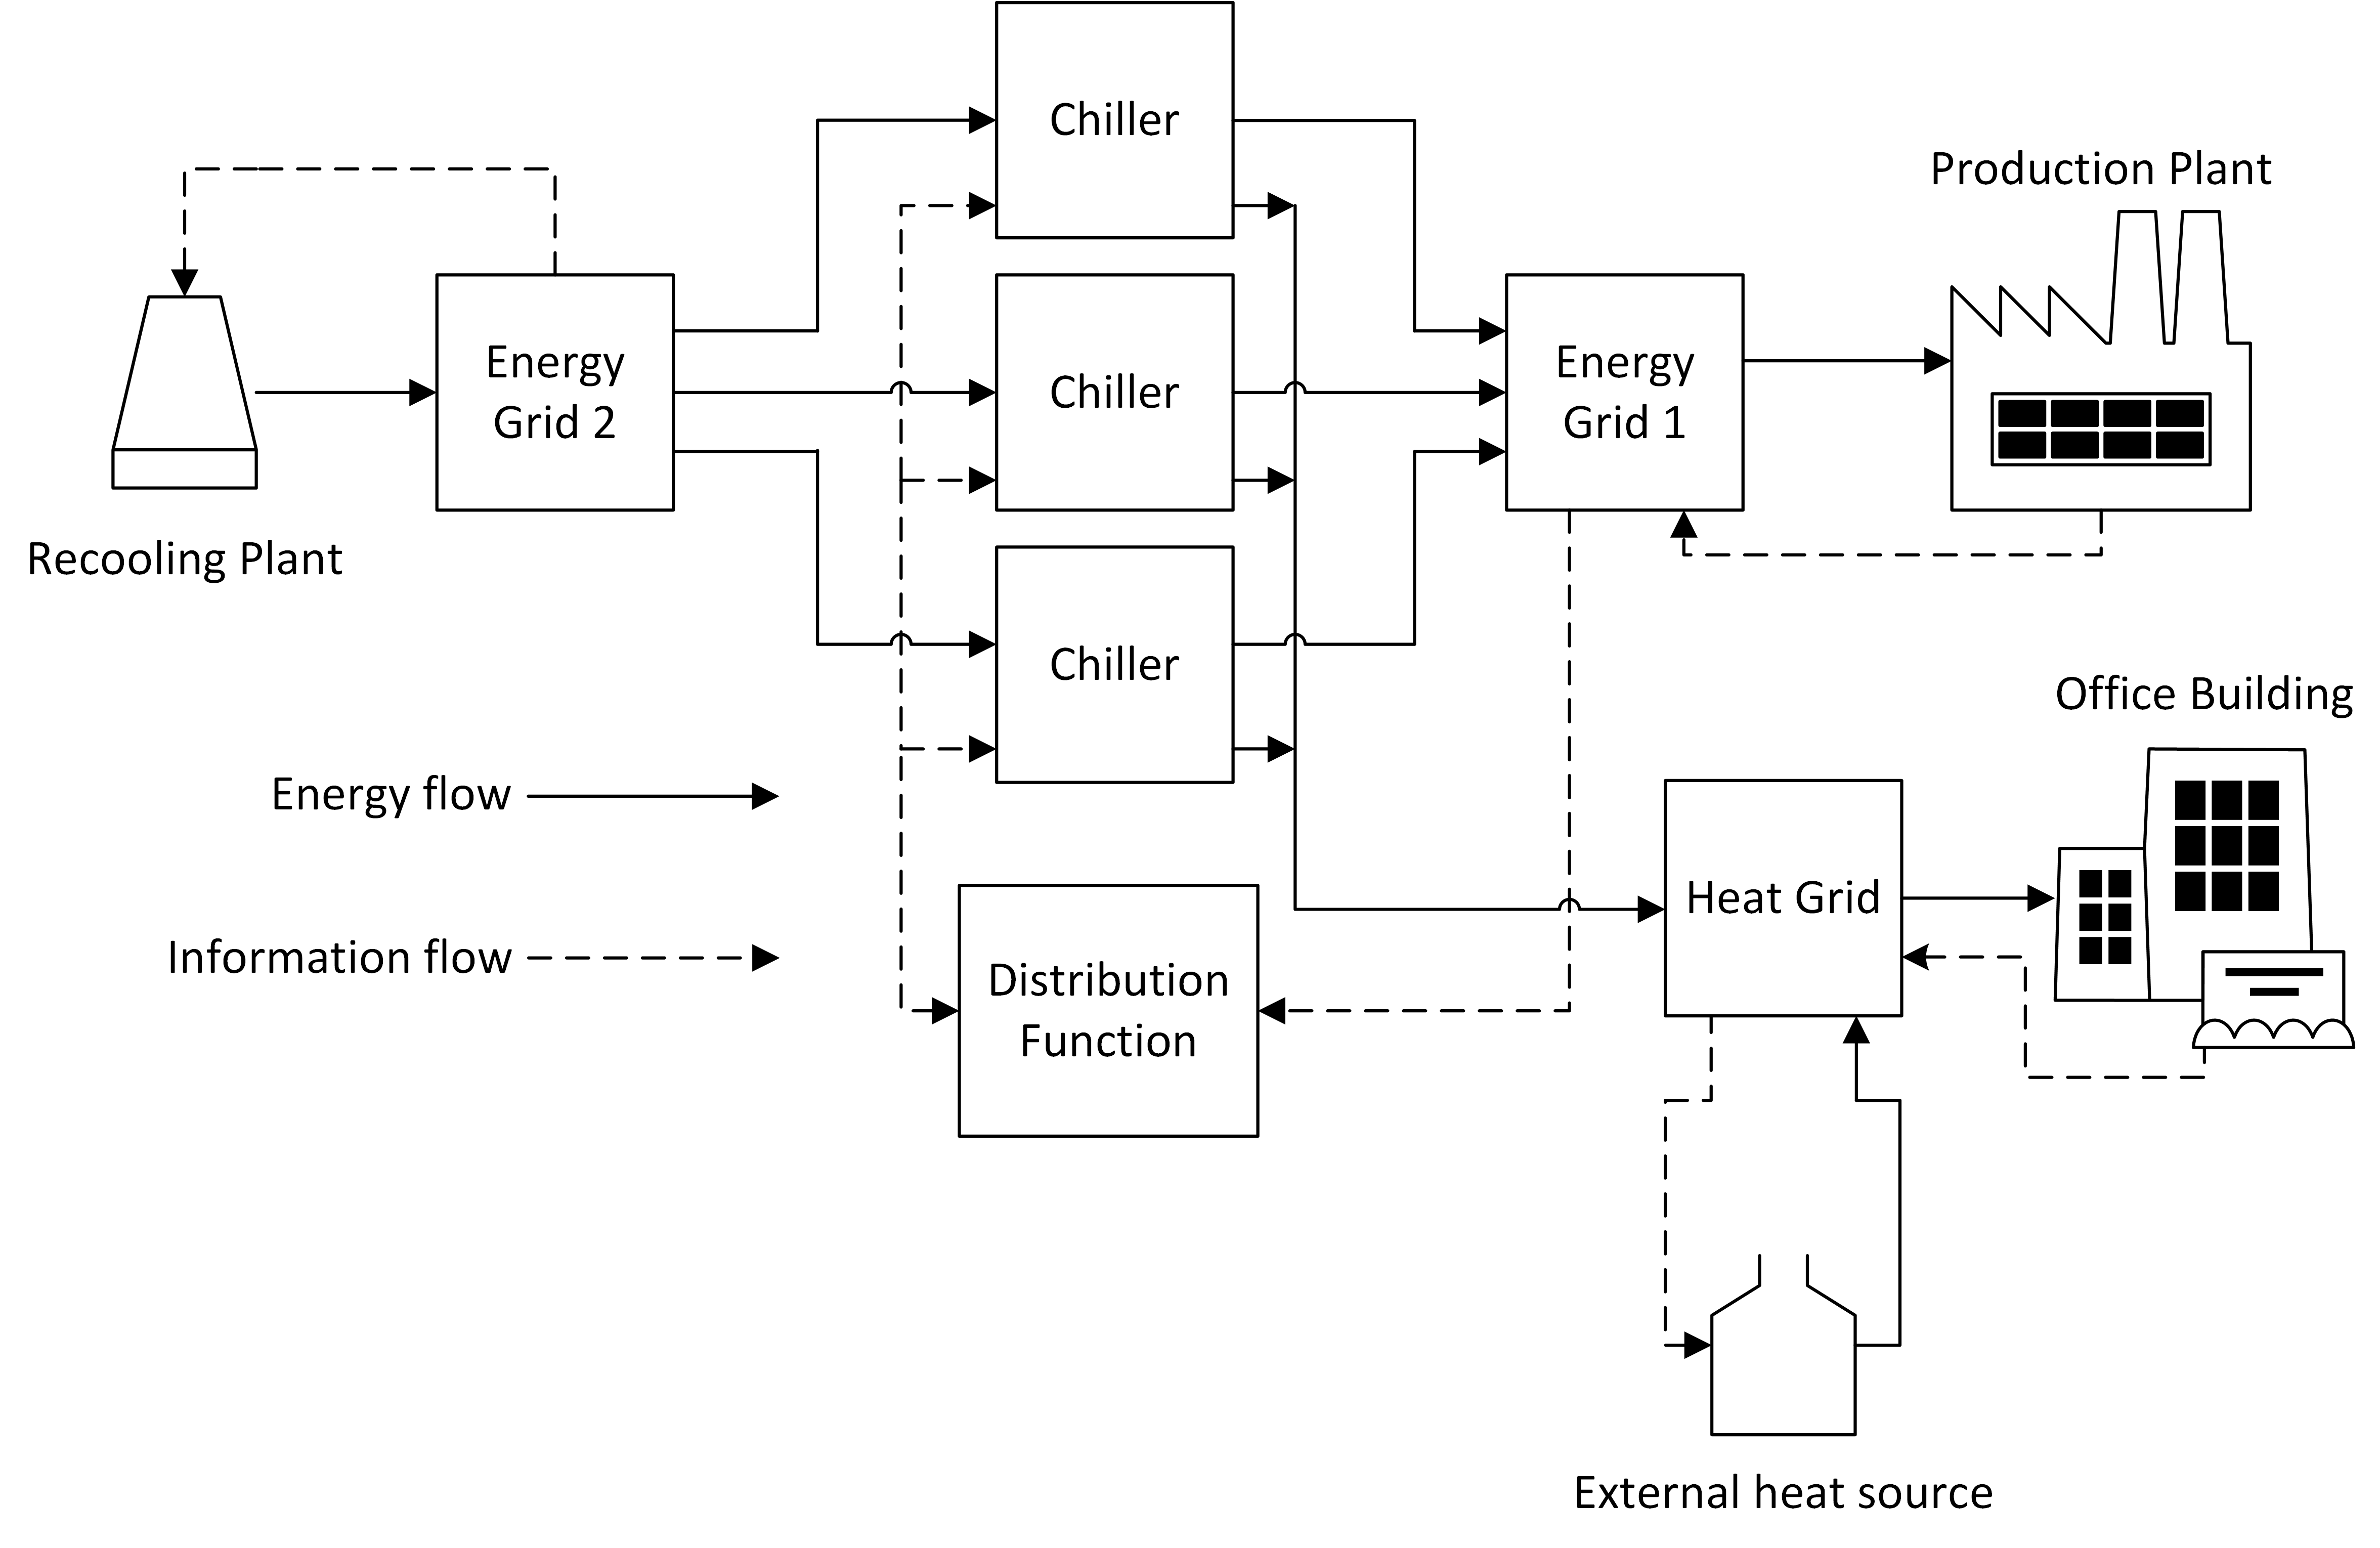
\includegraphics[width=21pc]{figures/modelstructure}}
	\caption{Overview of the model strucure.}
\end{figure}

The model consists of two main components: the chillers and the energy grids. Both of them are not part of the standard library of AMESIM and had to be written in C for the simulation. There are two types of flows between the components: information flow and energy flow (figure 1). For the signal routing between the components it was possible to use the standard components from the AMSIM library “Signal, Control”. The energy flow can be interpreted physically as heat flow Q ̇. The production plant requires a negative heat flow for cooling. This is the main input to the simulation. This requirement is sent to the energy grid as an information flow. The energy grid fulfils the requirement by sending a negative heat flow to the production plant. As a consequence, the energy level in the grid changes. The derivative of the energy in the store of the energy grid is:

\begin{equation}
\begin{array}{@{}lcl}

\displaystyle 
\frac{\partial E}{\partial t} &=& 
\displaystyle 
\frac
{1}
{C}
\cdot \left
(\dot{Q}_{producer} - \dot{Q}_{consumer}\right)
\\[6pt]

\end{array}\vspace*{-12pt}
\end{equation}

C is the Capacity of the grid. It depends on the real parameters mass m in the grid and the specific heat capacity cp:

\begin{equation}
\begin{array}{@{}lcl}

\displaystyle 
C &=& 
\displaystyle 
m \cdot c_p
\\[6pt]

\end{array}\vspace*{-12pt}
\end{equation}

From the current energy level E in the grid, the temperature of the fluid can be calculated:

\begin{equation}
\begin{array}{@{}lcl}

\displaystyle 
T &=& 
\displaystyle 
\frac{E}
{m \cdot c_p}
+ T_0
\\[6pt]

\end{array}\vspace*{-12pt}
\end{equation}

The internal variable E is the controlled variable of the grid. It is controlled by a PI-Controller. Energy grid 1 is also able to send the information about the needed Q to the distribution function. The distribution function splits the requirement in several parts and sends the information to the chillers. This is done by comparing two variables: the required heat flow Q\textsubscript{e,r} from the energy grid and the currently produced heat flow Q\textsubscript{e} from the chillers. If less negative heat is produced than consumed, the distribution function starts the next chiller by increasing the intern variable mon by 1 where mon represents the number of chillers running currently. The sequence in which the chillers are started is defined in the priority list. To avoid starting a machine with less negative heat requirement than 100 kW, a hysteresis is used.

\begin{equation}
\begin{array}{@{}lcl}
\displaystyle 

m_{on} &=&  
\left\{ \begin{array}{lcl}
m_{on} + 1 & &,\ if\ \dot{Q}_{e} - \dot{Q}_{e,r} > Hyst \\ 
m_{on} - 1 & &,\ if\ \dot{Q}_{e} - \dot{Q}_{e,r} < -Hyst
\end{array}\right.

\\[6pt]
\end{array}\vspace*{-12pt}
\end{equation}


The chiller submodel uses the chilled water supply temperature (T\textsubscript{chws}) in energy grid 1 and the temperature leaving the condenser (T\textsubscript{cnds}) in energy grid 2 provided by the energy grids as an external input variable to calculate the actual efficiency of the chiller as descriped in Hydeman et al. (2002). 

The chiller submodel uses the following energy flows: P\textsubscript{el}, Q\textsubscript{c} as an external input and Q\textsubscript{e}, Q\textsubscript{hr} as an external output. The information flows used are: the temperatures in energy grid 1 T\textsubscript{chws} and the temperature in energy grid 2 T\textsubscript{cnds}. It is possible to simulate the heat recovery as well, if the chiller supports it. The recovered heat flow Q\textsubscript{hr} is fed into the heat grid, which provides the office buildings (see figure 1) with a heat flow.

Q\textsubscript{hr} depends on the evaporator loading conditions. That is why it is calculated using Q\textsubscript{e}. The heat recovery efficiency coefficient  $ \eta\textsubscript{1} $ was determined by linear regression analysis and the method of least squares.

\begin{equation}
\begin{array}{@{}lcl}
\displaystyle 

\dot{Q}_{hr} &=& \eta_{1}\dot{Q}_{e} 

\\[6pt]
\end{array}\vspace*{-12pt}
\end{equation}

By using the heat recovery systems of the chillers, the heat energy from external sources Q\textsubscript{h,net} is reduced. If the heat recovery systems provide more heat energy, than consumed, no heat from external sources is needed and Q\textsubscript{h,net}=0:

\begin{equation}
\begin{array}{@{}lcl}
\displaystyle 

\dot{Q}_{h,net} &=&  
\left\{ \begin{array}{lcl}
\dot{Q}_{h,gross} - \dot{Q}_{hr} & &,\ if\ \dot{Q}_{h,gross} > \dot{Q}_{hr} \\ 
0 & &,\ if\ \dot{Q}_{h,gross} < \dot{Q}_{hr}
\end{array}\right.

\\[6pt]
\end{array}\vspace*{-12pt}
\end{equation}

To emit the heat of the chillers to the environment, a recooling plant is used. The recooling plant uses a very simple submodel: a maximum possible heat flow Q\textsubscript{cmax} to the environment is declared as a real parameter. If the required cooling energy flow Q\textsubscript{c} (sent as an information flow from the energy grid, and back to the grid as an energy flow) from the chillers is higher than Q\textsubscript{cmax}, not enough heat can be emitted to the environment and the temperature Tcnds in energy grid 2 rises. This influences CAPFT and EIRFT in the chillers as shown above.
The same effects occur when the requirement of negative heat flow Q\textsubscript{e,r} exceeds the maximum possible heat flow Q\textsubscript{e} from the chillers. The energy level in grid 1 decreases and the temperature T\textsubscript{chws} rises. The simulation considers this dynamic behaviour of the grids and the effects on the chillers.

\section{Optimization}
Based on the analysis of the model errors, 9 chillers were selected for optimization (Table 3). Since the cooling power required for the production is volatile throughout the day, a switch-on sequence is set on a daily basis. Based on this order, chillers will be turned on as needed. Since the efficiency of the chiller is highly dependent on the part load ratio as well as on the chilled water supply temperature (T\textsubscript{chws}) and the temperature leaving the condenser (T\textsubscript{cnds}), daily data recorded in the past can be used as a guide for the optimal operating strategy of the current demands. Due to the 9! ≈ 3.6E9 possibilities a genetic algorithm was chosen to find a time-efficient optimum.

The sequence of turning on the chillers is the degree of freedom of the optimizer and is determined in a priority vector. It has 9 entries. Every entry of the vector is assigned to a machine. An example for a vector is given here:

\begin{equation}
\begin{array}{@{}lcl}

\displaystyle 
\vec{p} &=& 
\displaystyle 
\left(8,2,4,9,6,7,5,3,1\right)
\\[6pt]

\end{array}\vspace*{-12pt}
\end{equation}

The vector can be read as follows: machine 8 is switched on first, then machine 2, then machine 4 and so on. Every entry in the priority vector is a natural number in the range from 1 to 9 and is unique. The simulation software doesn´t support vectors as a regular input for a genetic algorithm optimization process so a list of all possible vectors, that match the requirements, is predefined. The optimizer modifies the line number of the vector list to choose a vector. The result of the optimization process is the line number which contains the optimal vector.
Before the optimization starts a fitness function f has to be declared. The main goal of the fitness function is to evaluate a solution. The fitness function includes all relevant variables, the simulation calculates. Also, there is a weighting factor for every part of the function. In the optimization process the optimizer tries to minimize the fitness function.

\begin{equation}
\begin{array}{@{}lcl}

\displaystyle 
f &=& 
\displaystyle 
\omega_{1}P_{el,r} + \omega_{2}Q_{h,net}
\\[6pt]

\end{array}\vspace*{-12pt}
\end{equation}

The fitness function consists of two main parts: the first part is weighted with $ \omega_{1} $ and considers the electrical energy consumption P\textsubscript{el,r}. The second part is weighted with $ \omega_{2} $ and considers the heat energy consumption from external sources Q\textsubscript{h,net}. The heat energy consumption from external sources is calculated as the difference between the required heat energy and the heat provided by the chillers with heat recovery system (see section model implementation).
By setting the weight factors, different goals can be pursued. To perform an optimization of the energy consumption in the scenario, all factors can be set to 1. Then the optimizer directly minimizes the consumed energy in the scenario. Another goal could be the optimization of the costs. If both weighting factors are set to the energy prices for electricity and heat, the costs can be calculated directly from the fitness value and the optimizer minimizes the costs. Another use case is to reduce the impact on the environment by minimizing the CO2-Emmissions. Detailed information about the sources of electric and heat energy is required. The weighting factors can be set depending on the emitted CO2 by producing 1 kWh electric energy and 1 kWh heat energy.
Detailed information about the sources of electric and heat energy is required. The weighting factors can be set depending on the emitted CO2 by producing 1 kWh electric energy and 1 kWh heat energy.
The performance of the optimization process highly depends on the workload of the chillers. If the workload is high, a high number of chillers is running and the impact of the priority vector on the performance is reduced. If the workload is lower, there are more different switch-on sequences, so the optimizer has more degrees of freedom to reduce the fitness value. To evaluate the performance of the optimization process scenarios with high workload conditions and scenarios with low workload conditions are investigated separately (table 4).
In the first scenario the heat energy requirement weighting factor is set to 0. The electric energy conIsumption P\textsubscript{el,r},rlb is the only variable, effecting the fitness value. In the second scenario, the heat energy requirement weighting factor is set to 1. In this case, an optimization of the total energy consumption (electricity and heat) is performed. An overview of the used weighting and cost factors is given in table 4.

\begin{table}[t]
	\caption{weight factors and part load ratio for the scenarios}
	\begin{tabular*}{\hsize}{@{\extracolsep{\fill}}@{\hskip6pt}lll@{\hskip6pt}lll@{\hskip6pt}lll@{\hskip6pt}
			lll@{\hskip6pt}lll@{\hskip6pt}lll@{\hskip6pt}lll@{\hskip6pt}lll@{\hskip6pt}lll@{\hskip6pt}}
		\toprule
		scen. & \multicolumn{2}{l}{optimized}  & 
		T\textsubscript{chws}  & T\textsubscript{cnds} 
		& Q\textsubscript{e,r} & PLR & Q\textsubscript{h,gross} 
		& $\omega\textsubscript{1} $ & $\omega\textsubscript{2} $\\
		& \multicolumn{2}{l}{values} & ({\it{\degree C}}) & ({\it{\degree C}})& ({\it{kWh}}) &  ({\it{\%}}) & ({\it{kWh}})\\
		&  P\textsubscript{el,r} &  Q\textsubscript{h,net}\\
		\colrule
		1 & X & & 7.8 & 25.1 & 4.7E5 & 84.4 & 61375 & 1 & 0\\
		2 & X & & 7.2 & 24.3 & 2.0E5 & 35.9 & 86722 & 1 & 0\\
		3 & X & X & 7.2 & 25.1 & 4.7E5 & 84.4 & 61375 & 1 & 1\\
		4 & X & X & 7.8 & 24.3 & 2.0E5 & 35.9 & 86722 & 1 & 1\\
		\botrule
	\end{tabular*}
\end{table}

Table 5 shows the electric energy consumption of a simulated optimized priority vector compared to measured data. A reduction can be achieved with both workload (PLR) conditions. The reduction ratio highly depends on the workload. A higher workload leads to less optimization potential. It must be mentioned that there is still an error up to 28\% in energy prediction in the chiller models.
Scenario 3 and 4 are the same with the heat recovery systems included in the fitness function. So there are two main variables that effect the fitness value: P\textsuperscript{el,r} and Q\textsubscript{h,net}. Because of the influence of Q\textsubscript{h,net} to the fitness value, the reduction ratio is even higher, than without heat recovery. The results also depend on the operation strategy of the chillers while the measure data sets were recorded.

\begin{table}[t]
	\caption{Optimization performance}
	\begin{tabular*}{\hsize}{@{\extracolsep{\fill}}@{\hskip6pt}lll@{\hskip6pt}lll@{\hskip6pt}lll@{\hskip6pt}
			lll@{\hskip6pt}lll@{\hskip6pt}lll@{\hskip6pt}lll@{\hskip6pt}lll@{\hskip6pt}lll@{\hskip6pt}}
		\toprule
		scen. & PLR & \multicolumn{2}{l}{energy use ({\it{kWh}})}  & reduction \\
		& ({\it{\%}}) & with optimization & without optimization & ({\it{\%}})\\

		\colrule
		1 & 84.4 & 104592 & 89038 & 14.87\\
		2 & 35.9 & 53958 & 35094 & 34.96\\
		3 & 84.4 & 115672 & 90295 & 21.94\\
		4 & 35.9 & 70351 & 41473 & 41.05\\

		\botrule
	\end{tabular*}
\end{table}

\section{Conclusion}

\section{References}
\bibliography{Data_based_optimization}   % name your BibTeX data base
\bibliographystyle{spmpsci}      % mathematics and physical sciences
\end{document}

%%
%% End of file `procs-template.tex'.
